% Journal Article
% LaTeX Template
% Version 2.0 (February 7, 2023)
%
% This template originates from:
% https://www.LaTeXTemplates.com
%
% Author:
% Vel (vel@latextemplates.com)
%
% License:
% CC BY-NC-SA 4.0 (https://creativecommons.org/licenses/by-nc-sa/4.0/)
%
% NOTE: The bibliography needs to be compiled using the biber engine.
%
%%%%%%%%%%%%%%%%%%%%%%%%%%%%%%%%%%%%%%%%%

%----------------------------------------------------------------------------------------
%	PACKAGES AND OTHER DOCUMENT CONFIGURATIONS
%----------------------------------------------------------------------------------------

\documentclass[
	letterpaper, % Paper size, use either a4paper or letterpaper
	12pt, % Default font size, can also use 11pt or 12pt, although this is not recommended
	unnumberedsections, % Comment to enable section numbering
	twoside, % Two side traditional mode where headers and footers change between odd and even pages, comment this option to make them fixed
]{LTJournalArticle}

\addbibresource{bibliography.bib} % BibLaTeX bibliography file

\runninghead{Final Project} % A shortened article title to appear in the running head, leave this command empty for no running head

\footertext{\textit{Final Project} (MICS/DATSCI 266, Summer 2025)} % Text to appear in the footer, leave this command empty for no footer text

\setcounter{page}{1} % The page number of the first page, set this to a higher number if the article is to be part of an issue or larger work

%----------------------------------------------------------------------------------------
%	TITLE SECTION
%----------------------------------------------------------------------------------------

\usepackage[title,toc,titletoc]{appendix}
\usepackage{titlesec}
\usepackage{lscape}
\usepackage{fontawesome}


\title{Manipulative Language Detection in LLM-Crafted
Phishing Attacks
}  % Article title, use manual lines breaks (\\) to beautify the layout}

% Authors are listed in a comma-separated list with superscript numbers indicating affiliations
% \thanks{} is used for any text that should be placed in a footnote on the first page, such as the corresponding author's email, journal acceptance dates, a copyright/license notice, keywords, etc
\author{
	Karl-Johan Westhoff \\
	email \href{mailto:kjwesthoff@berkeley.edu}{kjwesthoff@berkeley.edu} \\
    Neha Dhage \\
	email \href{mailto:neha_dhage@ischool.berkeley.edu}{neha_dhage@ischool.berkeley.edu}
}


% Affiliations are output in the \date{} command
\date{UC Berkeley School of Information \\
MIDS Course 266 Summer 2025 Section 2 (Natalie Ahn) \\
}

% % Full-width abstract
% \renewcommand{\maketitlehookd}{%
% 	\begin{abstract}
% 		\noindent Lorem ipsum dolor sit amet,rta porttitor.
% 	\end{abstract}
% }

%----------------------------------------------------------------------------------------
\setcounter{tocdepth}{5}
\setcounter{secnumdepth}{5}
\usepackage[title]{appendix}

\begin{document}
\maketitle % Output the title section
%----------------------------------------------------------------------------------------
%	ARTICLE CONTENTS
%----------------------------------------------------------------------------------------
\section{Introduction}
The human factor remains central in cyber attacks. The 2024 Verizon DBIR report  notes that 68\% of breaches involve the human element, with phishing as a key contributor. With LLM tools, bad actors can now craft highly convincing phishing messages that evade traditional detection.
This project investigates whether NLP models can detect manipulative language—specifically, text designed to influence actions not in the reader's best interest.

Machine learning (ML) models like Naive Bayes and basic neural networks are widely used to filter email traffic for spam (which is an abundant problem). However, they are often limited to detecting specific words or obvious patterns. Newer approaches combine lightweight ML filtering with resource-heavy NLP methods for cases that are not clearly categorized by simpler filtering. Since phishing often exploits human psychology through language, this study focuses on detecting manipulative language and whether such detection may improve defenses against phishing. Although the focus is on cybersecurity, manipulative language also appears in areas such as coercive or abusive communication, highlighting its broader relevance. Our approach first models manipulation using the “Mental Manip” dataset, then explores its potential for phishing detection.

\section{Literature}
Salloum et al. [3] provide an overview of current ML and NLP methods used for phishing detection, which forms the foundational context for this project.
Suhaima et al. [4] trained models like BERT on spam data, whereas our focus will be on specifically detecting manipulative language.
Wang et al. [2] created a data set that targets dialogue manipulation, which will serve as our primary training set.
Al-Subaiey et al. have compiled a large corpus of emails in [6] from various datasets, under phishing specific email body texts; this will be used for attempts to detect phishing texts.

\section{Datasets}
Labeled data sets focused on manipulation are rare. Most of the research has come from psychology, which provides insight into the techniques used for manipulation. Most existing data sets suitable for NLP applications are concerned with hate speech and abusive language, which has been a hot topic in relation to online chat forums.

\subsection{The MentalManip Dataset}
Wang et al. [2] introduced the "MentalManip" dataset, published on hugging face[5]. The dataset is based on 4,000 fictional dialogues from online movie scripts. The data is labeled with a detailed manipulation taxonomy in three dimensions.

\begin{figure}[!htp] % Single column :figure	
	\centering
	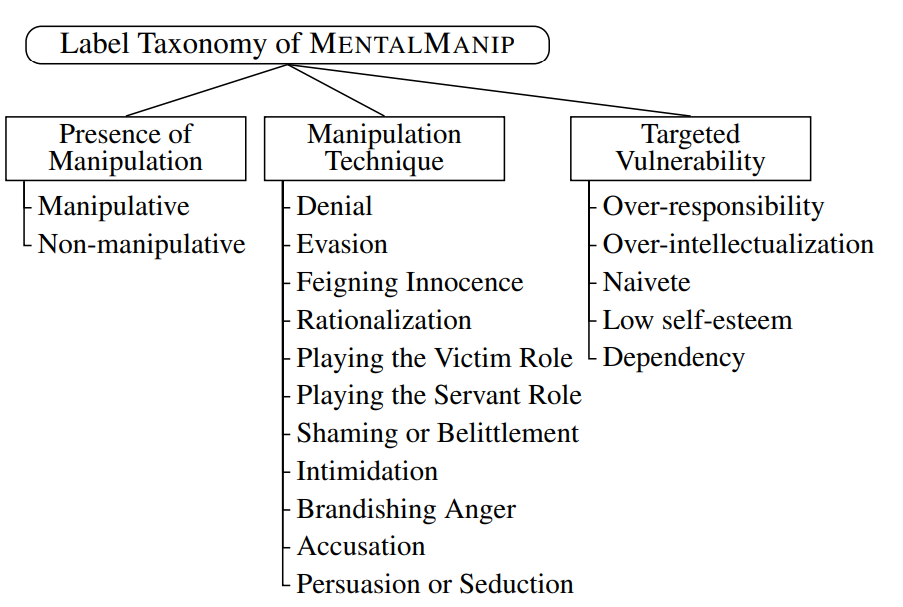
\includegraphics[width=0.5\textwidth]{Taxonomy.png}
	\caption{Taxonomy}
	\label{fig:Taxonomy}
\end{figure}




\subsection{Training Dataset}
The model will be trained on a dataset generated by Wang et al. \cite{MentalManip} which is based on 4000 labeled dialogues from films.\\

\subsection{Evaluation Dataset}
We will use data sets with labeled phishing emails in combination with results from previous models.

\section{Methods}
We will build an inference model that can detect manipulated emails based on a deep neural network with transformer architecture.

\section{Evaluation}
Our main interest is to investigate if the model can extend existing phishing detection systems by detecting manipulating language in the emails. We will to look at false negative results from previous models, to see if the detection of manipulative text captures emails that were previously missed.








%----------------------------------------------------------------------------------------
%	 REFERENCES
%----------------------------------------------------------------------------------------
\clearpage
\printbibliography % Output the bibliography
%----------------------------------------------------------------------------------------

%----------------------------------------------------------------------------------------
%	 Appendices
%---------------------------------------------------------------------------------------


%\begin{appendices}
%	\onecolumn
%
%	\section{Appendix}
%
%
\end{document}
